\documentclass[12pt]{article}
\title{Expense CLI: A Command-Line Expense Management Program}
\author{Kyle Dormer (S1802423)}
\date{January 13, 2019}
\usepackage{graphicx}
\usepackage{listings}
\usepackage{hyperref}
\usepackage{float}
\usepackage{lscape}


\begin{document}
  \pagenumbering{gobble}
  \maketitle
  \tableofcontents
  \newpage
  \pagenumbering{arabic}

  \section{Introduction}
  This piece of software is a command-line expense management tool. Its intended purpose is to allow the user to enter their income and their expenses and to have them stored and tracked for them. More specifically, the objectives of the software are that the user should be able to:
  \begin{itemize}
    \item Enter their monthly income, be it from single or from multiple sources.
    \item Set an overall monthly budget as well as a budget for categories of expense.
    \item Enter their expenses based on expense categories.
    \item Add new expense categories.
    \item View an exense report in terms of day/week/month/year and also with respect to a category.
    \item Generate and export a graph of their expenses in \textit{PDF} format.
    \item The expense report should should inform the user when they are over/under budget for a specific category in a specific month.
    \item The expense report should also display the average expense per category.
    \item These objectives should be achieved using a backend \textit{SQLite} database and with the \textit{Pandas} and \textit{Matplotlib} modules.
  \end{itemize}
  In retrospect to the development process, all of these objectives have been successfully implemented and achieved relatively smoothly and without issue. The biggest problems faced throughout the development of the software involved averaging the expenses of the user while generating the expense report. Furthermore, displaying the user's expenses in a nicely formatted fashion in a command-line environment proved difficult, as opposed to implementing a \textit{GUI} solution. The format was solved by designing an algorithm that makes use of Python's concept of \textit{list comprehension} in synergy with the inbuilt \textit{any()} function.
  \section{Design of System}
  \subsection{Design Paradigm}
  First and foremost, the design of the software is based upon the \textit{procedural} programming paradigm, derived from the \textit{imperative} paradigm.
  This can very much be reflected in the structure of the codebase. The program functions by the \textit{\_\_main\_\_} module making a call to the \textit{main()} function or \textit{procedure}, which in turn make calls to other functions which also make calls to other functions. An example of this can be observed within \textit{expcli.py}.
    \begin{lstlisting}[language=Python, caption=An example of procedural program design from \textit{expcli.py}, captionpos=b]
    option_choice = get_user_option([])

    if option_choice[0] == 1:
        get_income()

    elif option_choice[0] == 2:
        monthly_budget = get_monthly_budget([])
        sql.store_monthly_budget(monthly_budget[0])

    elif option_choice[0] == 3:
        expense = get_expense()
        sql.store_expense(expense)

    elif option_choice[0] == 4:
        categories = get_categories([])
        sql.store_categories(categories)

    elif option_choice[0] == 5:
        date = get_expense_date([])
        expenses = get_display_expenses('day', date[0], None)
        display_expenses(expenses)
    \end{lstlisting}
  As shown in Listing 1, the program obtains the user's choice for which option to take. Depending on the user's choice, the \textit{control flow} of the program is determined by making a function call to the function that corresponds with the user's choice. In fact, when combined with \textit{recursion}, this is how the entirety of the program functions; the user enters their option, the corresponding function calls are made, and then the user enters another option \textit{ad infinitum}.

  The procedural paradigm was chosen in the design of this program due to its focus on using \textit{variables}, \textit{data structures} and \textit{functions} to design and carry out algorithmic tasks. Whereas, for example, the \textit{object-oriented} design paradigm focuses on conceptualising real world concepts as objects that contain both data and methods to interact with said data. In the context of this program, user expenses and input are stored as data structures, more specifically as lists of dictionaries. Therefore, using procedurally designed functions to interact with this data makes more sense. Furthermore, object-oriented programing is often less efficient than procedural programming\cite{luca}, and with the relatively simple nature of the data involved in this program (expenses have only 4 properties), object-oriented was not deemed necessary nor favourable. 

  \subsection{Modular Programming}
  In combination with the procedural paradigm, the technique of \textit{modular programing} has also been focused upon throughout the design of this program.
  There are multiple reasons for this design choice. 

  Firstly, splitting the program into individual modules that each handle one area of functionality effectively \textit{encapsulates} complexity. Therefore, once a module has been implemented and thoroughly tested, it can be reused by I or another programmer without knowing how it works. All the knowledge required to use it would be its purpose, its arguments (if it has any) and its output.
  An example of this can be observed many times throughout the codebase of the program, although most notably in the usage of the \textit{exptools} module.

  \begin{lstlisting}[language=Python, caption=An example of encapsulation achieved via modular programming in \textit{expcli.py}, captionpos=b]
    def get_monthly_budget(budget_var):

      monthly_budget = input('Enter monthly budget: ')

      if ex.validate_input(monthly_budget, 1, 18, str):
          try:
              monthly_budget = float(monthly_budget)
              budget_var.append(monthly_budget)

          except (Exception):
              ex.print_important('Invalid number, please try again!')
              get_monthly_budget(budget_var)
      else:
          ex.print_important('Invalid number, please try again!')
          get_monthly_budget(budget_var)

      return budget_var
    \end{lstlisting} 

  This function's purpose is to recursively collect a monthly budget from the user and makes use of the \textit{validate\_input()} and \textit{print\_important()} functions from the \textit{exptools} module, although in this context its module object is defined as \textit{ex} for shorthand use.

  Secondly, as alluded to in the first point, modular programming allows for very effective \textit{code reuse}. Indeed, this was in fact the original reasoning behind the creation of modular programming, first implemented in \textit{ALGOL 68-R} in 1970.\cite{algol}. As can be seen in Listing 2, the \textit{validate\_input()} function can be called (reused) whenever needed.

  Thirdly and finally, modular programming achieves \textit{separation of concerns}. This means that each concern (or aspect of functionality) of the program belongs to a self-contained module. This ties in with the first point in that it allows the code of modules to change completely and still work perfectly as long as their expected inputs and outputs remain the same to interface properly with the rest of the program.
  \subsection{Recursion}
  Most of the functions, especially functions that gather user input, in this program shall be \textit{recursive}. This involves a function calling itself to achieve a purpose. This is very useful in obtaining user input which must be validated for length or type. One objective of the program is to allow the user to enter their expenses. This will involve the expense's category, expense's date and the expense's amount; a string, string (or \textit{datetime} object) and a float respectively. Furthermore, the strings must be between a minimum and maximum length. However, it is unlikely that the user will perfectly enter the desired input in a proper fashion each time. Therefore if validation of the user's input fails, the program should alert the user to the correct format of input and prompt them again.
  An algorithm for this could be implemented as pseudocode as such.
    \begin{lstlisting}[caption=An example pseudocode algorithm to inefficiently obtain valid user input, captionpos=b]
      WHILE TRUE:
        GET input
        IF VALIDATE input FALSE:
          GET input
    \end{lstlisting}

  However, this algorithm is flawed in that the user may not enter the input in the correct format even after being prompted, and to deal with this the \textit{if} block would have to keep nesting under itself \textit{ad infinitum}.
  Therefore, instead of having an infinite loop and a potentially infinite control structure, the function could simply call itself again if the user does not enter the input correctly. This would be resource efficient as it would only be called as much as needed and would simplify and reduce the lines of code needed to be written.
  The pseudocode for this newly imagined algorithm can be expressed in Listing 4.
    \begin{lstlisting}[caption=A correct\, recursive algorithm to obtain valid user input, captionpos=b]
      SUB get_input:
        GET input
        IF VALIDATE input TRUE:
          RETURN input
        ELSE:
          get_input
    \end{lstlisting}

  An implementation of the Listing 4 algorithm can be observed in Listing 2.
  This algorithm will be repurposed throughout the program for whenever the user needs to input data (expenses, expense categories, income sources, and monthly budget).

  \subsection{Algorithms for the Objectives}
  The purpose of this section is to specify algorithms that achieve each objective set out in the specification.
  \subsubsection{Control Flow}
  The overall algorithm has been alluded to previously. It will display the options to the user and procedurally carry out the desired option and then recursively allow the user to enter another option (unless the user opts to exit the program).

  The flowchart for this algorithm can be expressed as such.
    \begin{figure}[H]
      \centering
      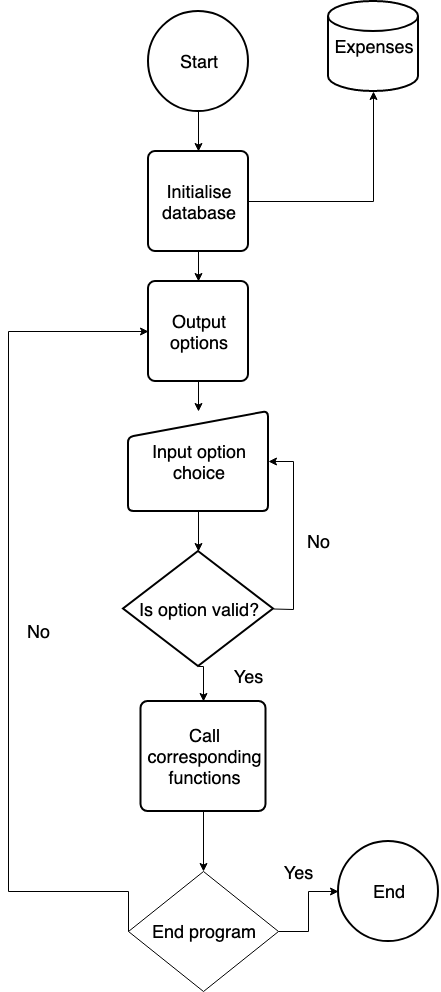
\includegraphics[scale=0.4]{overall_program_flow.png}
      \caption{The overall control and execution flow of the program.}
    \end{figure}

  \subsubsection{Enter Monthly Income}
  To obtain the user's monthly income, the algorithm will use recursion as discussed previously. Furthermore, each source of income will be stored in a data structure formed of a list of dictionaries. For instance, the user enters two income sources \textit{'Salary'} and \textit{'Side Job}, the former with an income of \textit{£1000} and the latter with \textit{£250}. Assuming the input is valid, the final data structure would be a list containing two dictionaries. The dictionary would have a key for the name and a key for the income of the source. To store these in the database, a \textit{foreach} loop can be used to loop through each dictionary in the list and gather the income.
  The algorithm can be expressed in flowchart format as such.
  \begin{figure}[H]
    \centering
    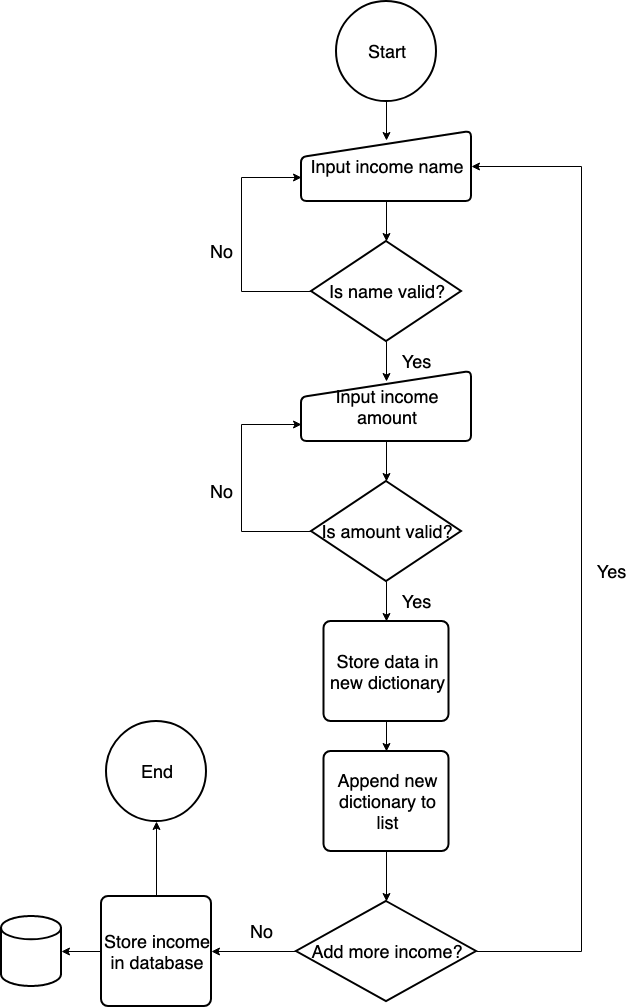
\includegraphics[scale=0.4]{monthly_income.png}
    \caption{An algorithm to obtain and store the user's monthly income.}
  \end{figure}

  \subsubsection{Set Overall Monthly Budget}
  Setting the overall monthly budget is a relatively simple process. Firstly, the program will take the user's desired budget as input using the same aforementioned recursive algorithm. Then, it will update the \textit{Budget} field in the database for each month.
  This can be expressed in pseudocode.
  \begin{lstlisting}[caption=An algorithm to set the overall monthly budget., captionpos=b]
    SUB get_budget:
      INPUT budget
      IF VALIDATE budget TRUE:
        UPDATE Budget in Month WITH budget
      ELSE:
        get_budget
  \end{lstlisting}

  \subsubsection{Enter Expenses Based on Categories}
  To allow the user to enter expenses based on categories, the program will get all expense categories from the database and then allow them to choose which category the expense belongs to. It will also get the date of the expense and the amount. Then, the expense will be stored in a data structure consisting of a list of dictionaries, each dictionary containing the amount, date and category.
  The algorithm for this can be expressed in Python as such.
  \begin{lstlisting}[language=Python, caption=An algorithm to collect expenses from the user., captionpos=b]
  def get_expense():
    expense_category = get_category_choice([])
    expense_date = get_expense_date([])
    expense_amount = get_expense_amount([])

    if (expense_category and expense_date) and expense_amount:
        expense = {'category': expense_category[0],
                  'date': expense_date[0], 'amount': expense_amount[0]}

        return expense
  \end{lstlisting}

  The functions \textit{get\_category\_choice()}, \textit{get\_expense\_date()} and \textit{get\_expense\_amount()} will all follow the recursive input algorithm detailed previously. For illustration, the code for \textit{get\_expense\_amount()} can be shown as such.

  \begin{lstlisting}[language=Python, caption=Source code for \textit{get\_expense\_amount()}, captionpos=b]
  def get_expense_amount(amount_arr):
    
    amount = input('Enter expense amount: ')

    if ex.validate_input(amount, 1, 12, str):
        try:
            amount = float(amount)
            amount_arr.append(amount)
        except (Exception):
            ex.print_important(
                'Invalid amount! Please enter a valid number!')
            get_expense_amount(amount_arr)
    else:
        ex.print_important('Invalid amount! Please enter a valid number!')
        get_expense_amount(amount_arr)

    return amount_arr
  \end{lstlisting}

  \subsubsection{Add New Categories}
  Adding new categories remains similar to the previous algorithms. The categories will be collected recursively from the user. Then, the user will have the option of inputting a monthly budget for the category. If yes, the budget is inputted and validated and if no, the budget is set to a Python signal object of \textit{None}.

  \subsubsection{View Expense Report}
  To display an expense report to the user, the \textit{Pandas} module is used to tabulate the data.
  The user has the option to see an expense report by day/week/month/year and category. For dates, there will be functions that will get the date specified and check which day/week/month/year it belongs to. Then, each expense that matches this day/week/month/year will be put into an expense array/list. Then, this expense list will be passed to a \textit{Pandas} data frame. Then, using the \textit{to\_string()} method of a data frame object, the data will be sorted by category and displayed in table format to the user.

  \subsubsection{Generate Graph of Expenses in PDF Format and Display Average and Total Expense for Category}
  The program will use the \textit{matplotlib} module to achieve this. The average and total expenses for each expense category will be fetched from the database. This will be done by pasing an array of all expenses to a function belonging to the \textit{exptools} module. The source code for this function can be observed below in Listing 8. The algorithm takes an array of expense \textit{tuples} as an argument. Then, it uses Python's \textit{any()} function and an iterator to check if the expense category has already been added to the \textit{categories} list. If it hasn't already been added, it is appended to the list in the form of a dictionary with keys for the category name, expense total, expense average and category budget. Once this operation has been completed, the categories list is looped through using a \textit{foreach} loop. For each category in the categories list, the budget for the category is retrieved from the database and added to the corresponding dictionary key. Then, an expense counter variable is declared. All expenses in the expense array will then be iterated through and checked to see if they belong to the current category being looped through. If the expense indeed does belong to the category, the category's total expense becomes equal to its current value added to the new expense's amount and the expense count has one added to it. Then, the category's \textit{mean} average expense is obtained by dividing the category's total expense by the number of expenses within that category, held within the expense count variable.
  Then, the category's total expense is checked to see if it is lower or higher than the category's set monthly budget. If the category has no budget, it is set to 'None' by handling the \textit{exception} that occurs.
  Once this process has finished, the list of dictionaries is passed to a \textit{Pandas} data frame object. This object can then be passed to a \textit{matplotlib} bar chart and exported to PDF or it can be displayed in the expense report in tabular format to the user.

  \begin{landscape}
    \begin{lstlisting}[language=Python, caption=Source code for \textit{get\_average\_expenses().}, captionpos=b]
      def get_average_expenses(expense_array):
      categories = []

      for expense in expense_array:
          if not any(category['Category'] == expense[2] for category in categories):
              categories.append(
                  {'Category': expense[2], 'Total': 0, 'Average': 0, 'Budget': None})

      for category in categories:
          expense_count = 0
          budget = sql.get_budget(category['Category'])

          for expense in expense_array:
              if expense[2] == category['Category']:
                  category['Total'] += expense[3]
                  expense_count += 1

          category['Average'] = category['Total'] / expense_count

          try:
              if category['Total'] > budget[0]:
                  category['Budget'] = 'Over'
              else:
                  category['Budget'] = 'Under'
          except (TypeError):
              category['Budget'] = 'None'

          expense_count = 0

      return categories
      
    \end{lstlisting}
  \end{landscape}

  \subsection{Database}
  The design of the database can be observed in the following entity-relationship diagram.

  \begin{figure}[H]
    \centering
    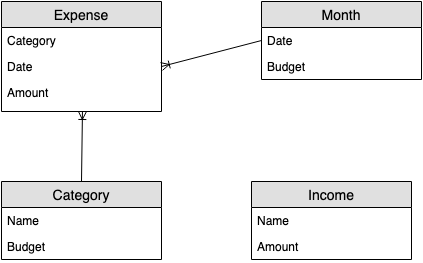
\includegraphics[scale=0.7]{database.png}
    \caption{Entity relationsip diagram for the proposed database.}
  \end{figure}

  All operations involving the database will be contained in a module named \textit{expsql.py}.

  \section{Testing the System}
  \section{Demonstrating the System}

  \appendix
  \section{User Guide}
  \section{Code}
  \section{Test Suites}

  \begin{thebibliography}{9}
    \bibitem{luca}
    Cardelli, Luca (1996),
    \textit{Bad Engineering Properties of Object-Oriented Languages},
    Digital Equipment Corporation Systems Research Center
    Sourced from: \url{http://lucacardelli.name/Papers/BadPropertiesOfOO.html},
    Accessed: [22nd January 2020].

    \bibitem{algol}
    C. H. Lindsey (University of Manchester) \&
    H. J. Boom (Mathematisch Centrum, Amsterdam),
    \textit{A Modules and Separate Compilation Facility for ALGOL 68},
    Sourced from: \url{http://archive.computerhistory.org/resources/text/algol/ACM_Algol_bulletin/1061719/p19-lindsey.pdf},
    Accessed: [22nd January 2020].


  \end{thebibliography}

\end{document}
